\begin{frame}{Quick Questions}
  \begin{itemize}
    \item How many of you did NOT bring smartphones with you?
    \item Is your smartphone powered off now?
    \item Where is your smartphones now?
  \end{itemize}
  \begin{block}{Unique Natures of Smartphones}
    \begin{enumerate}
      \item Carried with you.
      \item Always on.
      \item Mostly idle.
    \end{enumerate}
  \end{block}
  \vspace*{5mm}
  {\LARGE Ideal vantage point for network monitoring!}
\end{frame}

\begin{frame}{Why "Ideal"?}
  \begin{enumerate}
    \item \textbf{Carried with YOU.}
      \begin{itemize}
        \item Capture the real user's RF conditions and experience.
        \item As opposed to site suveys or statically deployed sniffers.
      \end{itemize}
    \item \textbf{Always on.}
      \begin{itemize}
        \item Provide \textit{continous} stream of measurements.
        \item As opposed to laptops.
      \end{itemize}
    \item \textbf{Mostly Idle.}
      \begin{itemize}
        \item Avoid interrupting normal usage.
      \end{itemize}
    \item \textbf{Additional Benifits}
      \begin{itemize}
        \item No additional hardware cost.
        \item Easy to deploy (app markets).
      \end{itemize}
  \end{enumerate}
\end{frame}

\begin{frame}{Our Proposal at a Glance}
  \begin{block}{Use smartphones for}
    \textbf{Long-term large scale network monitoring.}
    \begin{itemize}
      \item Network health, performance, etc.
    \end{itemize}
    \textbf{Short-term local spectrum management.}
    \begin{itemize}
      \item Snif the spectrum on behalf of nearby devices.
      \item Help with channel assigment, rate adaption, etc.
    \end{itemize}
  \end{block}
\end{frame}

\begin{frame}{PocketSniffer System}
  \begin{figure}
    \centering
    \begin{tikzpicture}
      \node[anchor=south west,inner sep=0] at (0,0)
      {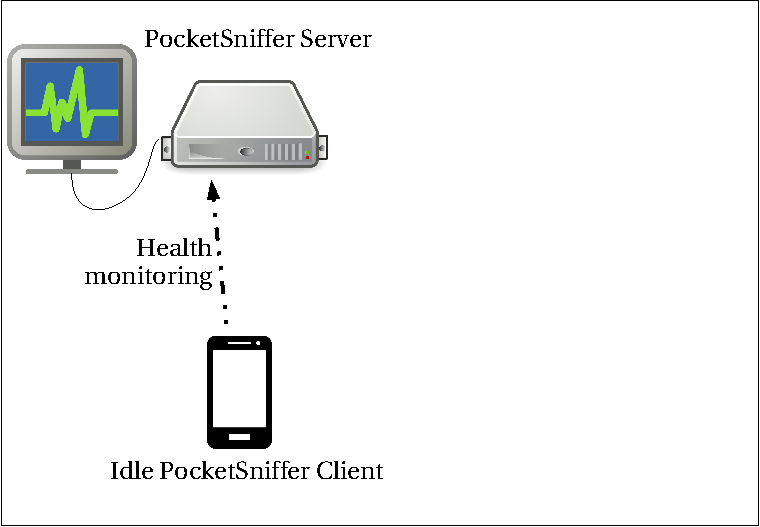
\includegraphics[width=0.8\textwidth]{system-1}};
      \pause
      \node[anchor=south west,inner sep=0] at (0,0)
      {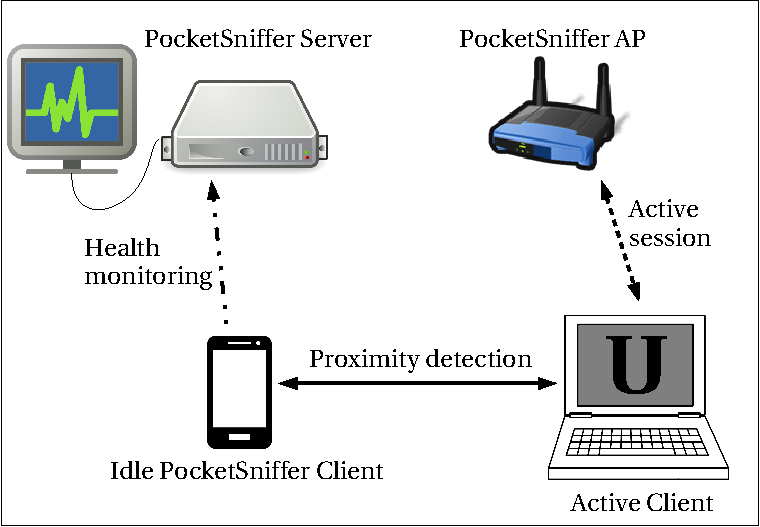
\includegraphics[width=0.8\textwidth]{system-2}};
      \pause
      \node[anchor=south west,inner sep=0] at (0,0)
      {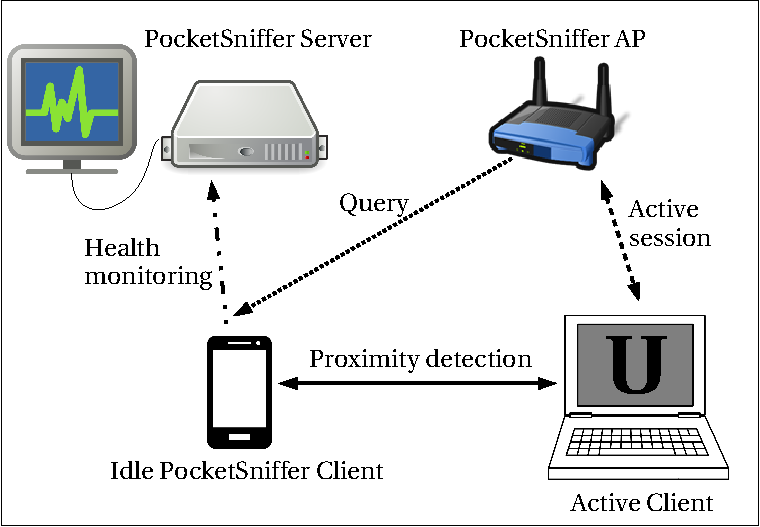
\includegraphics[width=0.8\textwidth]{system-3}};
      \pause
      \node[anchor=south west,inner sep=0] at (0,0)
      {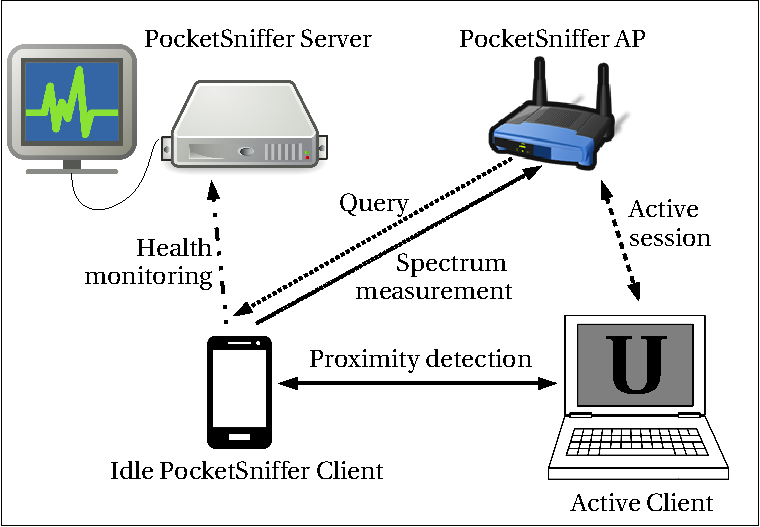
\includegraphics[width=0.8\textwidth]{system-4}};
    \end{tikzpicture}
  \end{figure}
\end{frame}
